% TODO:














%%%%%%%%%%%%%%%%%%%%%%%%%%%%%%%%%%%%%%%%%
% Beamer Presentation
% LaTeX Template
% Version 1.0 (10/11/12)
%
% This template has been downloaded from:
% http://www.LaTeXTemplates.com
%
% License:
% CC BY-NC-SA 3.0 (http://creativecommons.org/licenses/by-nc-sa/3.0/)
%
%%%%%%%%%%%%%%%%%%%%%%%%%%%%%%%%%%%%%%%%%

%----------------------------------------------------------------------------------------
%	PACKAGES AND THEMES
%----------------------------------------------------------------------------------------

\documentclass{beamer}

\mode<presentation> {

% The Beamer class comes with a number of default slide themes
% which change the colors and layouts of slides. Below this is a list
% of all the themes, uncomment each in turn to see what they look like.

%\usetheme{default}
%\usetheme{AnnArbor}
%\usetheme{Antibes}
%\usetheme{Bergen}
%\usetheme{Berkeley}
%\usetheme{Berlin}
%\usetheme{Boadilla}
%\usetheme{CambridgeUS}
%\usetheme{Copenhagen}
%\usetheme{Darmstadt}
%\usetheme{Dresden}
%\usetheme{Frankfurt}
%\usetheme{Goettingen}
%\usetheme{Hannover}
%\usetheme{Ilmenau}
%\usetheme{JuanLesPins}
%\usetheme{Luebeck}
\usetheme{Madrid}
%\usetheme{Malmoe}
%\usetheme{Marburg}
%\usetheme{Montpellier}
%\usetheme{PaloAlto}
%\usetheme{Pittsburgh}
%\usetheme{Rochester}
%\usetheme{Singapore}
%\usetheme{Szeged}
%\usetheme{Warsaw}

% As well as themes, the Beamer class has a number of color themes
% for any slide theme. Uncomment each of these in turn to see how it
% changes the colors of your current slide theme.

%\usecolortheme{albatross}
%\usecolortheme{beaver}
%\usecolortheme{beetle}
%\usecolortheme{crane}
%\usecolortheme{dolphin}
%\usecolortheme{dove}
%\usecolortheme{fly}
%\usecolortheme{lily}
%\usecolortheme{orchid}
%\usecolortheme{rose}
%\usecolortheme{seagull}
%\usecolortheme{seahorse}
%\usecolortheme{whale}
%\usecolortheme{wolverine}

%\setbeamertemplate{footline} % To remove the footer line in all slides uncomment this line
%\setbeamertemplate{footline}[page number] % To replace the footer line in all slides with a simple slide count uncomment this line

%\setbeamertemplate{navigation symbols}{} % To remove the navigation symbols from the bottom of all slides uncomment this line
}

\usepackage[utf8]{inputenc}
\usepackage[russian]{babel}
\usepackage{cmap}


\usepackage{verbatim}
\usepackage{fancybox}
\usepackage{ulem}
\usepackage{tikz}
\usetikzlibrary{positioning}
\usepackage{scalefnt}
\usetikzlibrary{arrows,shapes,positioning,shadows,trees,calc,backgrounds,fit,positioning}

\usepackage{graphicx} % Allows including images
\usepackage{booktabs} % Allows the use of \toprule, \midrule and \bottomrule in tables
\usepackage{textcomp}
\usepackage{listings}
\usepackage{color}
\usepackage{xcolor}
\usepackage{changepage}

\definecolor{mygreen}{rgb}{0,0.6,0}
\definecolor{mygray}{rgb}{0.5,0.5,0.5}
\definecolor{mymauve}{rgb}{0.58,0,0.82}

\lstset{ %
  backgroundcolor=\color{white},   % choose the background color; you must add \usepackage{color} or \usepackage{xcolor}
  basicstyle=\footnotesize,        % the size of the fonts that are used for the code
  breakatwhitespace=false,         % sets if automatic breaks should only happen at whitespace
  breaklines=true,                 % sets automatic line breaking
  captionpos=b,                    % sets the caption-position to bottom
  commentstyle=\color{mygreen},    % comment style
  deletekeywords={...},            % if you want to delete keywords from the given language
  escapeinside={\%*}{*)},          % if you want to add LaTeX within your code
  extendedchars=true,              % lets you use non-ASCII characters; for 8-bits encodings only, does not work with UTF-8
  frame=single,                    % adds a frame around the code
  keepspaces=true,                 % keeps spaces in text, useful for keeping indentation of code (possibly needs columns=flexible)
  keywordstyle=\color{blue},       % keyword style
  language=Octave,                 % the language of the code
  morekeywords={*,...},            % if you want to add more keywords to the set
  numbers=left,                    % where to put the line-numbers; possible values are (none, left, right)
  numbersep=5pt,                   % how far the line-numbers are from the code
  numberstyle=\tiny\color{mygray}, % the style that is used for the line-numbers
  rulecolor=\color{black},         % if not set, the frame-color may be changed on line-breaks within not-black text (e.g. comments (green here))
  showspaces=false,                % show spaces everywhere adding particular underscores; it overrides 'showstringspaces'
  showstringspaces=false,          % underline spaces within strings only
  showtabs=true,                  % show tabs within strings adding particular underscores
  stepnumber=1,                    % the step between two line-numbers. If it's 1, each line will be numbered
  stringstyle=\color{mymauve},     % string literal style
  tabsize=4,                       % sets default tabsize to 2 spaces
  %title=\lstname                   % show the filename of files included with \lstinputlisting; also try caption instead of title
}

\graphicspath{{./figures/}}

%----------------------------------------------------------------------------------------
%	TITLE PAGE
%----------------------------------------------------------------------------------------

\title[Обработка и исполнение запросов: лекция 4]{Обработка и исполнение запросов в СУБД (Лекция 4) \\~\\ Классические системы: введение в распределенные СУБД\\~\\ v4} % The short title appears at the bottom of every slide, the full title is only on the title page

\author{Георгий Чернышев} % Your name
\institute[ВШЭ] % Your institution as it will appear on the bottom of every slide, may be shorthand to save space
{
Высшая Школа Экономики \\ % Your institution for the title page
\medskip
\textit{chernishev@gmail.com} % Your email address
}
%\date{\today} % Date, can be changed to a custom date
\date{23 сентября 2020 г.}


\begin{document}

\begin{frame}
\titlepage % Print the title page as the first slide
\end{frame}

\begin{comment}
\begin{frame}
\frametitle{Overview} % Table of contents slide, comment this block out to remove it
\tableofcontents % Throughout your presentation, if you choose to use \section{} and \subsection{} commands, these will automatically be printed on this slide as an overview of your presentation
\end{frame}
\end{comment}

\begin{frame}
\frametitle{Распределенные СУБД I}

\begin{figure}[htb]
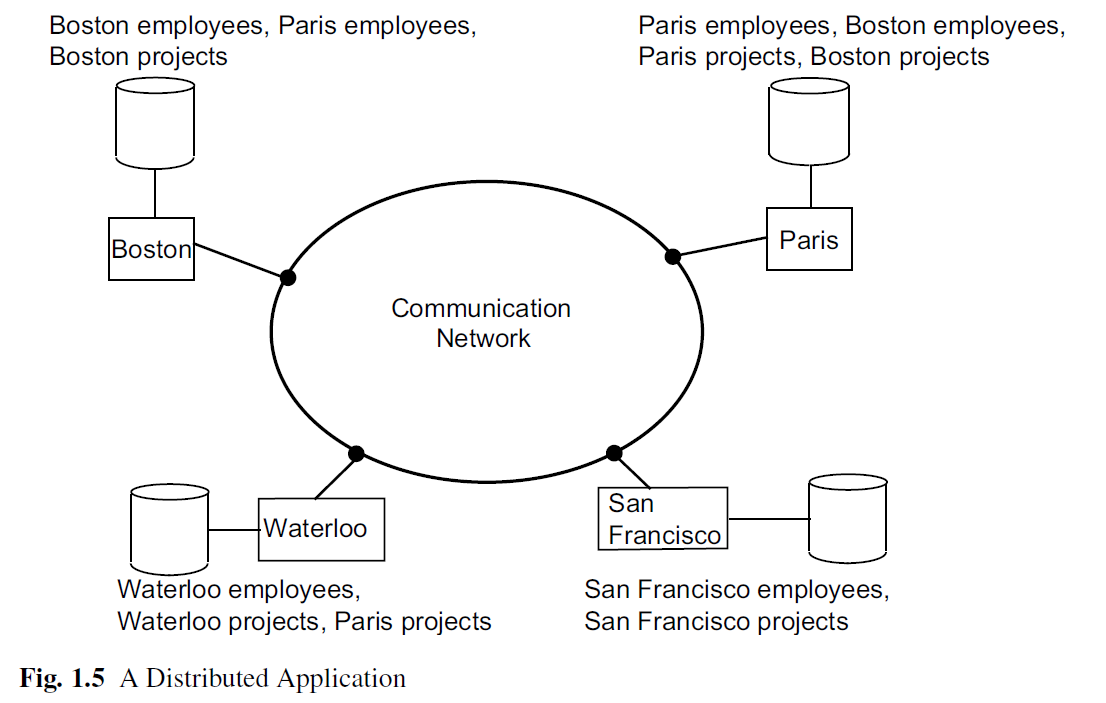
\includegraphics[width=\textwidth,height=0.50\textheight,keepaspectratio]{ozsu-1.png} 
\footnote{\tiny{Изображение взято из \cite{Ozsu2011}}}
\end{figure}
{\scriptsize
РСУБД \cite{Elnikety2009}: СУБД управляющая базой данных, данные которой подвергнуты фрагментированию и реплицированию, и находятся на нескольких, связанных друг с другом, узлах.
\\~\\
Основная цель РСУБД~--- ``спрятать'' физическую распределенность от клиентов. Клиенты работают с одной базой, видимой как единое целое;
}
\end{frame}


\begin{frame}
\frametitle{Распределенные СУБД II}

История:

\begin{itemize}
  \setlength\itemsep{1em}
  \item Появились в конце 70х, вместе с shared-nothing системами;
  \begin{itemize}
    \setlength\itemsep{1em}
    \item Нужда больших организаций иметь несколько офисов;
    \item Основная проблема в те годы: медленность сетей;
  \end{itemize}
  \item Первые системы, примеры \cite{Kian-Lee2009}:
\begin{itemize}
  \setlength\itemsep{1em}
  \item Исследовательские проекты: SDD-1 (Computer Corporation of America, 1980), Distributed INGRES (University of California at Berkeley, 1986), R*STAR (IBM, 1981); 
  \item Коммерческие продукты: INGRES/Star (1987), Oracle (1987), IBM продукты для интеграции разных версий DB2.
\end{itemize}


\end{itemize}

\end{frame}


\begin{frame}
\frametitle{Что может (и должна) дать РСУБД? I}

\alert{Транспарентность при управлении данными.}

\begin{figure}[htb]
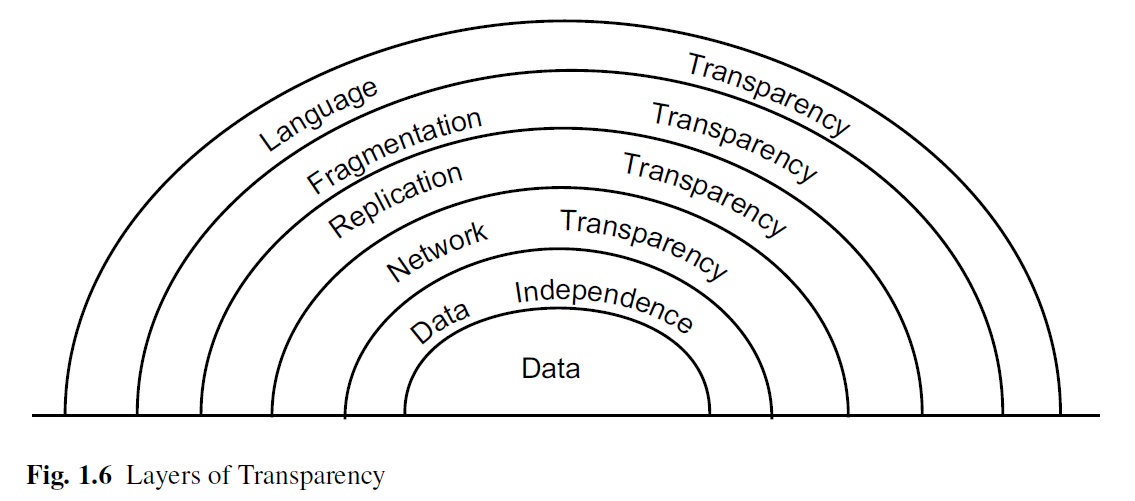
\includegraphics[width=\textwidth,height=0.80\textheight,keepaspectratio]{ozsu-2.png} 
\footnote{\tiny{Изображение взято из \cite{Ozsu2011}}}
\end{figure}

\end{frame}


\begin{frame}
\frametitle{Транспарентность в РСУБД}

Пользователь должен считать что работает с централизованной СУБД. Для этого надо обеспечить \cite{Ozsu2011}:
\begin{itemize}
  \item Транспарентность сети: 
  \begin{itemize}
    \item транспарентность локации;
    \item транспарентность имен;
  \end{itemize}
  \item Транспарентность фрагментирования данных;
  \item Транспарентность репликации данных;
  \item Языковую транспарентность.
\end{itemize}

В \cite{Kian-Lee2009} выделяется еще и транспарентность выполнения транзакций.

\end{frame}


\begin{frame}
\frametitle{Что может дать РСУБД? II}

Еще \cite{Ozsu2011}:
\begin{itemize}
  \setlength\itemsep{1em}
  \item Надежность посредством распределенных транзакций;
  \item Повышение производительности:
  \begin{itemize}
    \item локализация данных: 1) обработка только части данных и 2) меньше сетевые задержки;
    \item естественный параллелизм: 1) межзапросный и 2) внутризапросный;
  \end{itemize}
  \item Расширяемость системы;
  
\end{itemize}
\end{frame}

\begin{frame}
\frametitle{Фрагментирование данных}

Бывает:
\begin{itemize}
  \setlength\itemsep{1em}
  \item Горизонтальное, ``подклеиваем'' cнизу с помощью UNION;
  \item Вертикальное, ``подклеиваем'' сбоку с помощью JOIN;
  \item Смешанное.
\end{itemize}

Выбор оптимальной схемы фрагментирования это $NP$-трудная задача, обычно отдается на откуп администратору (ручной труд), вертикальное сложнее.\\~\\

Системы лучше поддерживают горизонтальное: PostgreSQL (набор горизонтальных фрагментов), Oracle (наведенное горизонтальное фрагментирование, partition by reference) и т.д.
\end{frame}

\begin{frame}
\frametitle{РСУБД, сложности}

РСУБД бывают:
\begin{itemize}
  \item Полностью реплицированные: на каждом узле есть вся база;
  \item Полностью фрагментированные: каждый узел содержит свой уникальный фрагмент, фрагменты попарно не пересекаются, объединение дает всю базу;
  \item Что-то среднее.
\end{itemize}

Основные исследовательские задачи связанные с РСУБД:
\begin{itemize}
  \item Как хранить данные?
  \item Как при обновлениях синхронизировать копии?
  \item Как осуществлять координацию и коммуникации между узлами при исполнении запроса?
\end{itemize}

\end{frame}

\begin{frame}
\frametitle{Компоненты РСУБД}

\begin{figure}[htb]
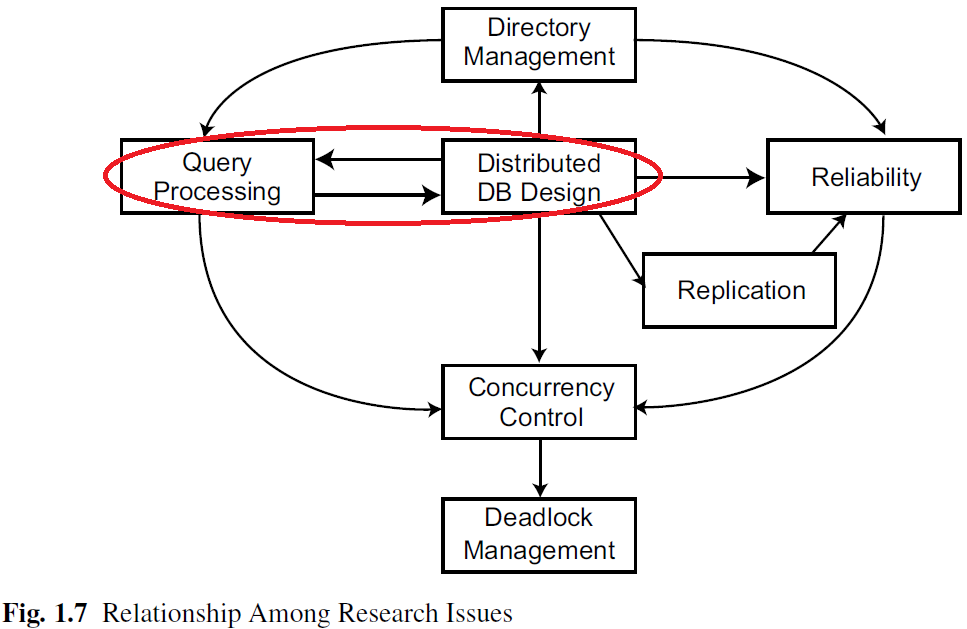
\includegraphics[width=\textwidth,height=0.80\textheight,keepaspectratio]{ozsu-3.png} 
\footnote{\tiny{Изображение взято из \cite{Ozsu2011}}}
\end{figure}

\end{frame}

\begin{frame}
\frametitle{Какие бывают РСУБД}

\begin{figure}[htb]
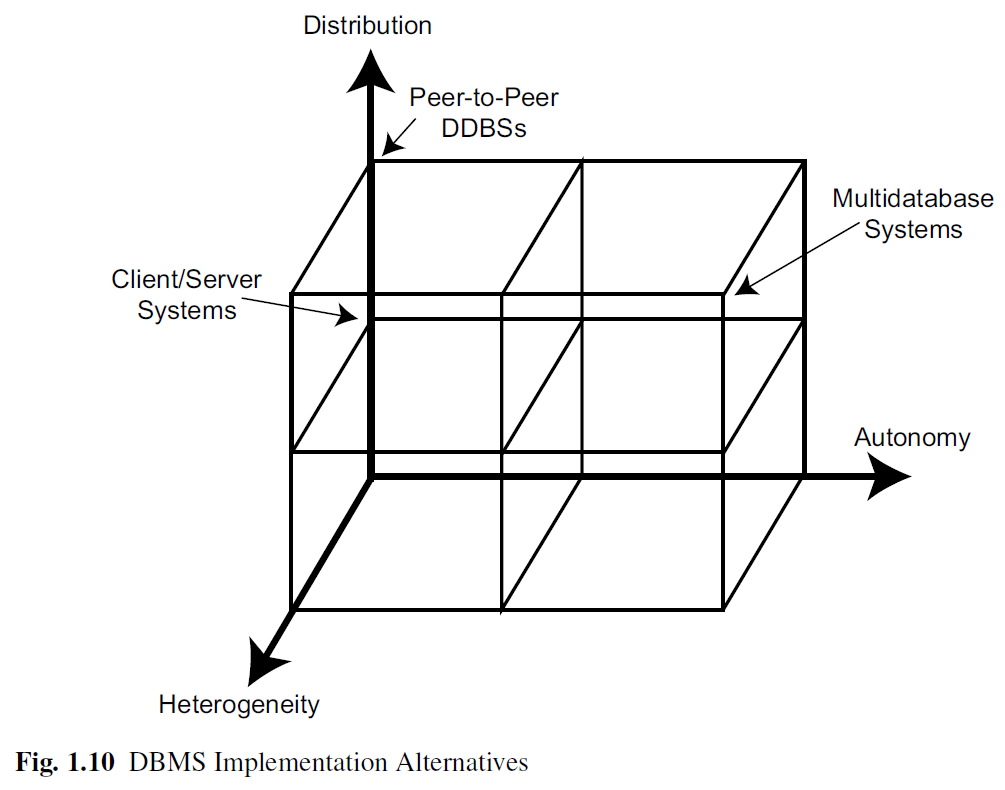
\includegraphics[width=\textwidth,height=0.80\textheight,keepaspectratio]{ozsu-4.png} 
\footnote{\tiny{Изображение взято из \cite{Ozsu2011}}}
\end{figure}

\end{frame}


\begin{frame}
\frametitle{Аспекты РСУБД: автономность I}
Автономность, в смысле автономности управления, не данных. Показывает насколько могут отдельные СУБД работать по отдельности.

Классические требования к автономности:
{\scriptsize
  \begin{itemize}
    \item Распределенная система не влияет на локальные операции отдельных СУБД;
    \item Выполнении глобальных запросов не влияет на способы выполнения и оптимизации локальных запросов;
    \item В случае добавления или выбывания отдельных СУБД консистентность работы РСУБД не должна страдать.
  \end{itemize}
}

Какая бывает автономность:
{\scriptsize
\begin{itemize}
  \item Автономность дизайна БД: СУБД-участники могут использовать любые модели данных и способы управления транзакциями;
  \item Автономность коммуникации: СУБД-участник решает какую информацию предоставлять другим СУБД или \alert{другому управляющему ПО};
  \item Автономность выполнения: СУБД-участник решает как выполнять свои транзакции.
\end{itemize}
}
\end{frame}

\begin{frame}
\frametitle{Аспекты РСУБД: автономность II}
Градации:
	\begin{itemize}
		\item Тесная интеграция~--- пользователю предоставляется единое видение базы, даже если она раскидана по локальным базам. Локальные базы не работают по-отдельности.
		\item Полуавтономная система~--- локальные системы могут работать независимо от наличия глобальной. Федерация баз~--- сами решают какие части делать доступными для пользователей других баз. Обычно требуют модифицикации кода. 
		\item Полностью изолированная система~--- stand-alone системы, друг о друге не знают.
	\end{itemize}

Это не единственные альтернативы, но самые популярные.

\end{frame}

\begin{frame}
\frametitle{Аспекты РСУБД: распределенность}

Распределенность именно в контексте управления данными.\\~\\

Типы систем:
  \begin{itemize}
    \setlength\itemsep{1em}  
    \item Клиент-серверная: управление данными на серверах, обеспечение пользовательского доступа~--- на клиентах;
    \item Peer-to-peer: нет различия между типами машин;
    \item Отсутствие распределенности.
  \end{itemize}

\end{frame}

\begin{frame}
\frametitle{Аспекты РСУБД: гетерогенность}

Гетерогенность:
  \begin{itemize}
    \setlength\itemsep{1em}  
    \item Хардварная;
    \item Сетевая;
    \item Моделей данных;
    \item Языков запросов;
    \item Протоколов управления транзакциями;
    \item ...
  \end{itemize}

В рассматриваемой классификации она либо есть, либо нет.

\end{frame}

% [allowframebreaks]
\begin{frame}
\frametitle{Основные типы РСУБД I}

Типы:
  \begin{itemize}
    \setlength\itemsep{1em}  
    \item (A0,D1, H0) клиент-сервер РСУБД;
    \begin{itemize}
      %\setlength\itemsep{1em}    
      \item Клиент-серверность: не процесс, а разделение машин;
      \item Появились в 90е;
      \item Сервер: основная работа;
      \item Клиент: Application Interface, UI, кеши данных, кешированные замки транзакций;
      \item модели: 
      \begin{itemize}
      	\item много клиентов - один сервер;
		\item много клиентов - много серверов;
      \end{itemize}
      \item много клиентов - много серверов:
      \begin{itemize}
	    \item тяжелый клиент~--- клиент сам выбирает куда подсоединяться когда надо, это упрощает код сервера но огружает клиентские машины;
	    \item легкий клиент~--- клиент помнит о ``домашнем'' сервере, сервер делает всю работу по взаимодействию c другими серверами;
	  \end{itemize}

      \item трехуровневая и многоуровневая архитектура.
    \end{itemize}

  \end{itemize}

\end{frame}

\begin{frame}
\frametitle{Клиент-серверная СУБД}

\begin{figure}[htb]
	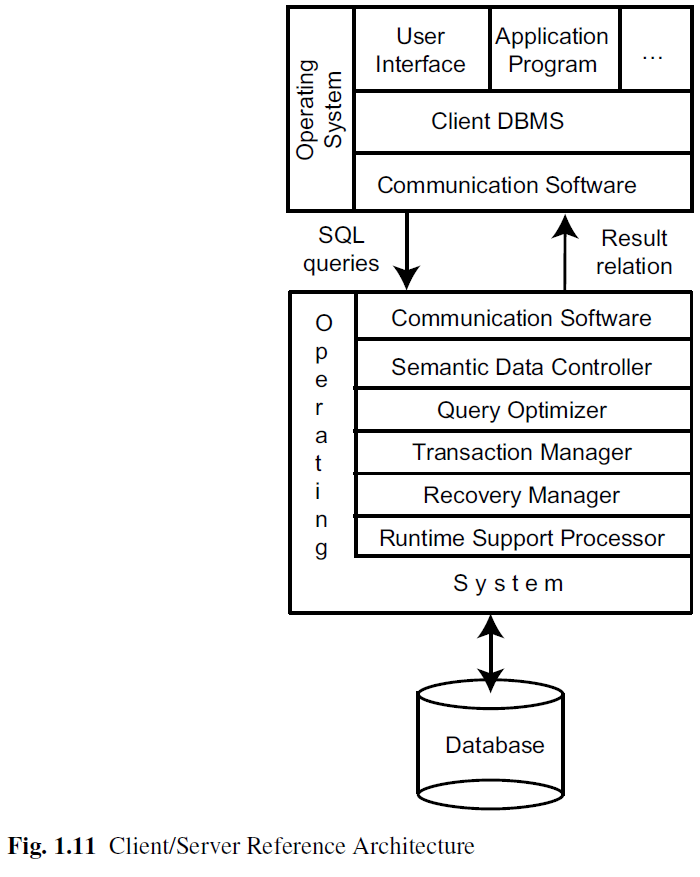
\includegraphics[width=\textwidth,height=0.80\textheight,keepaspectratio]{ozsu-7.png} 
	\footnote{\tiny{Изображение взято из \cite{Ozsu2011}}}
\end{figure}

\end{frame}

\begin{frame}
\frametitle{Трехуровневая архитектура I}

\begin{figure}[htb]
	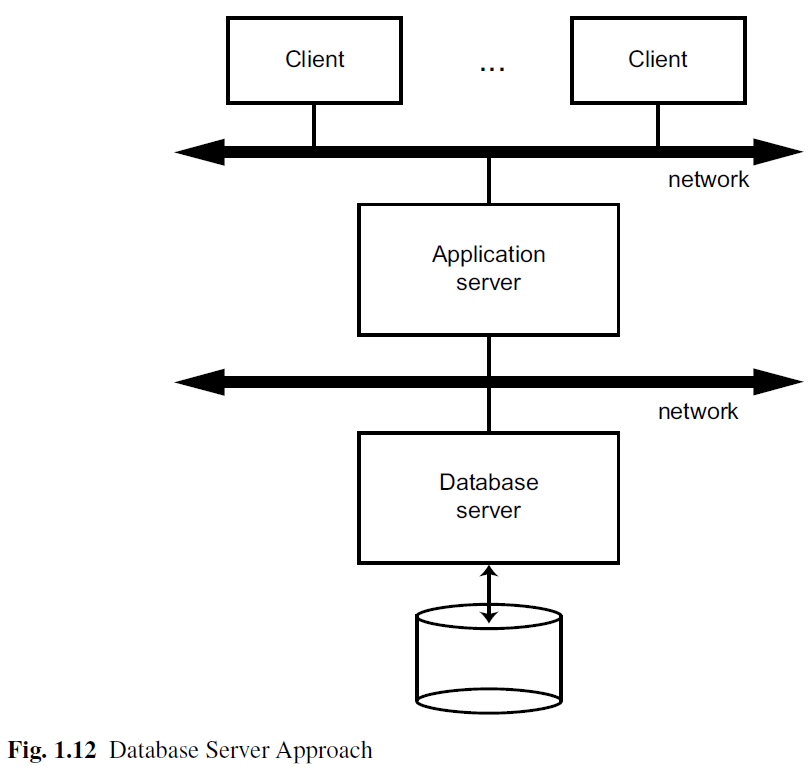
\includegraphics[width=\textwidth,height=0.80\textheight,keepaspectratio]{ozsu-8.png} 
	\footnote{\tiny{Изображение взято из \cite{Ozsu2011}}}
\end{figure}

\end{frame}

\begin{frame}
\frametitle{Трехуровневая архитектура II}

\begin{figure}[htb]
	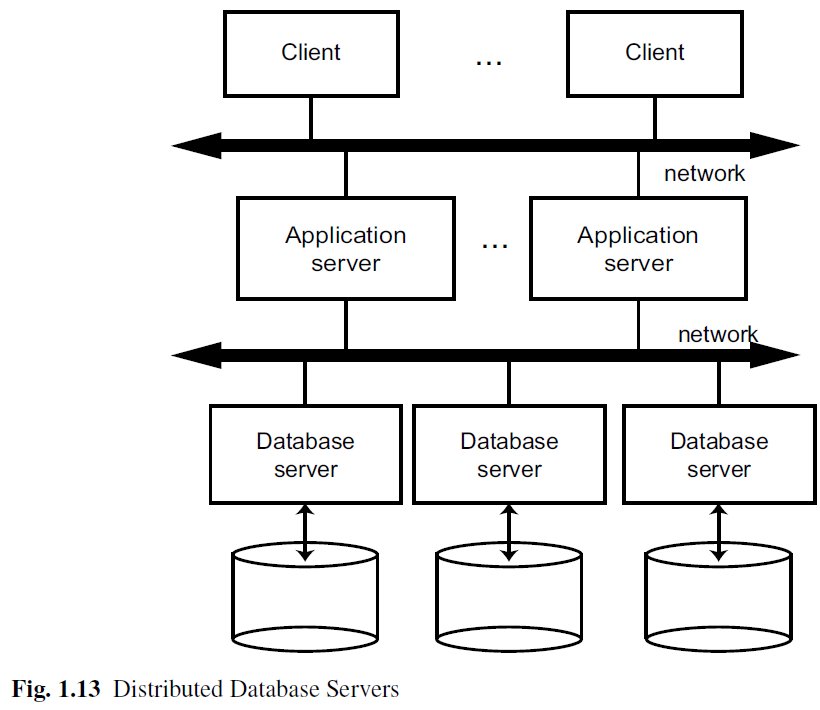
\includegraphics[width=\textwidth,height=0.80\textheight,keepaspectratio]{ozsu-9.png} 
	\footnote{\tiny{Изображение взято из \cite{Ozsu2011}}}
\end{figure}

\end{frame}


\begin{frame}
\frametitle{Основные типы РСУБД II}

Типы:
  \begin{itemize}
    \setlength\itemsep{1em}  
    \item (A0, D2, H0) Peer-to-Peer РСУБД;
    \begin{itemize}
      \setlength\itemsep{1em}    
      \item Два периода популярности: до 90-х и в нулевые;
      \item Машины не различаются между собой;
      \item local internal schema (LIS)~--- физическая организация на узлах может быть различной, поэтому ее надо описывать (на всех узлах);
      \item local conceptual schema (LCS) ~--- описывает фрагментирование и реплицирование на узле, объединение дает GCS;      
      \item global conceptual schema (GCS)~--- хранит общий вид логической структуры на всех узлах;
      \item external schema (ES)~--- для пользовательского доступа.
    \end{itemize}

  \end{itemize}

\end{frame}

\begin{frame}
	\frametitle{Пояснение про схемы}
	
	\begin{figure}[htb]
		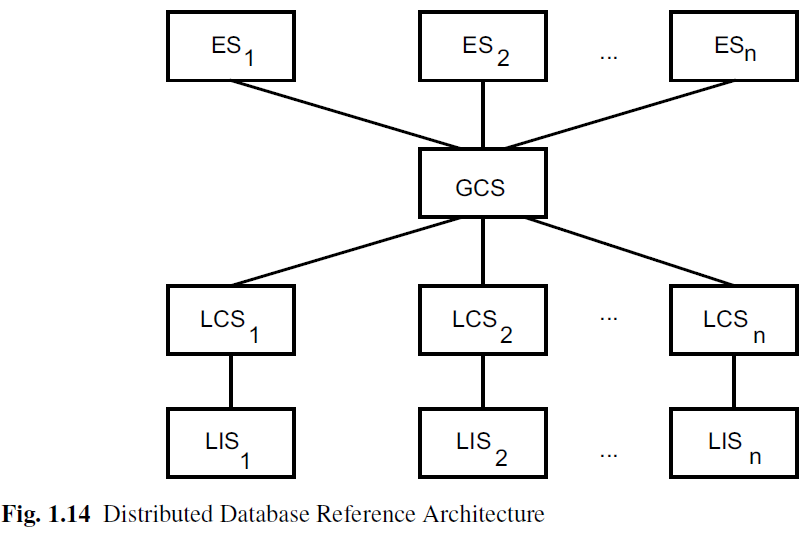
\includegraphics[width=\textwidth,height=0.80\textheight,keepaspectratio]{ozsu-10.png} 
		\footnote{\tiny{Изображение взято из \cite{Ozsu2011}}}
	\end{figure}
	
\end{frame}



\begin{frame}
\frametitle{Peer-to-Peer РСУБД}

\begin{figure}[htb]
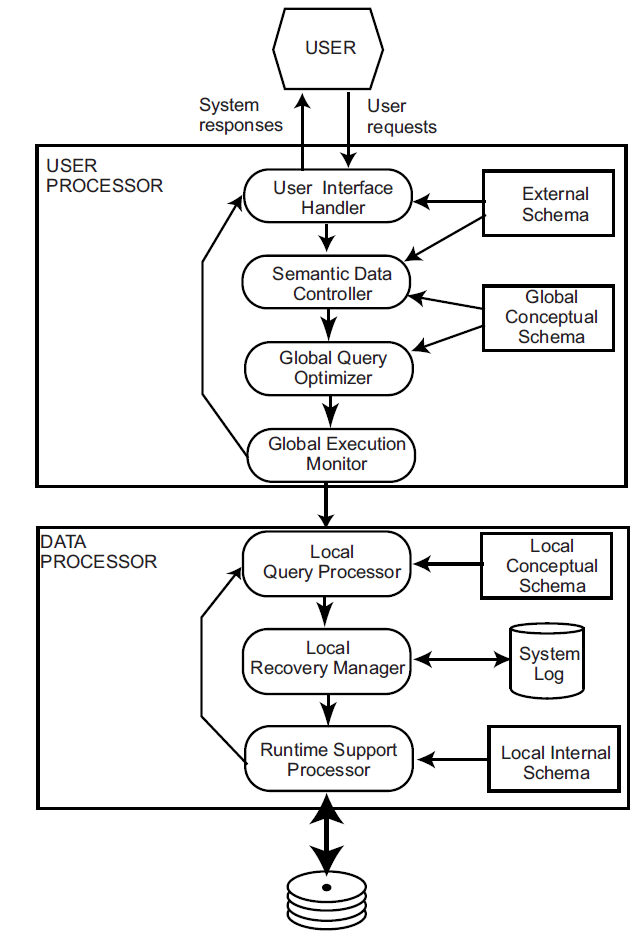
\includegraphics[width=\textwidth,height=0.80\textheight,keepaspectratio]{ozsu-5.png} 
\footnote{\tiny{Изображение взято из \cite{Ozsu2011}}}
\end{figure}

\end{frame}


\begin{frame}
\frametitle{Основные типы РСУБД III}

Типы:
  \begin{itemize}
    \item (A2, D2, H1) (p2p) гетерогенная мультибаза (интеграционная система, гетерогенная система).
    \begin{itemize}
    \setlength\itemsep{1em}      
      \item полностью автономны, отдельные СУБД друг о друге не знают;
      \item другое понятие глобальной базы данных, подмножество: то, что отдельные базы готовы выложить в общий доступ;
      \item GCS = $\cup$ ES участников или же \\GCS = $\cup$ часть LCS участников;
      %\item unilingual и multilingual мультибаза:\\
      %\underline{unilingual}~--- пользователь базы данных участника != пользователю всей системы, могут быть разные языки и модели данных.\\
      %\underline{multilingual}~--- пользователь отдельных баз может запрашивать данные на своем языке у глобальной базы. \alert{Тут в книге перепутано?}
      \item часто реализуются посредством mediator или middleware;
      \item иногда надо писать wrapper (обертку).
  \end{itemize}
\end{itemize}
\end{frame}

\begin{frame}
\frametitle{Устройство мультибазы}

\begin{figure}[htb]
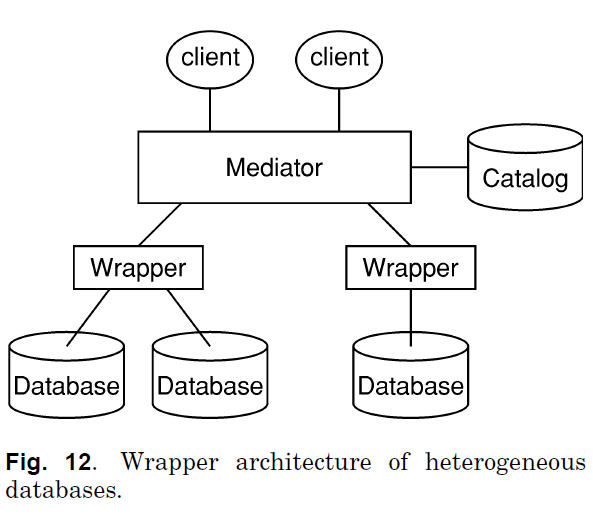
\includegraphics[width=\textwidth,height=0.75\textheight,keepaspectratio]{kossman-1.png} 
\footnote{\tiny{Изображение взято из \cite{Kossmann2000}}}
\end{figure}

\end{frame}

\begin{comment}

\begin{frame}[allowframebreaks]
\frametitle{РСУБД, сложности и частичные ответы~\cite{Elnikety2009}}

Основные исследовательские задачи связанные с РСУБД:
\begin{itemize}
  \item Как хранить данные?
  \begin{itemize}
    \item Принцип локальности данных $\longrightarrow$ увеличение количества реплик $\longrightarrow$ страдают апдейты;
    \item Ручной труд администратора по фрагментированию;
    \item Аллокация: статическая и динамическая, экономические модели;
  \end{itemize}
  \item Как при обновлениях синхронизировать копии?
  \begin{itemize}
    \item Протоколы кворума;
    \item Коммерческие системы используют ROWAA\\ $\longrightarrow$ семантика одной копии;
    \item Распространения обновлений: lazy и eager методы;
  \end{itemize}

    \item Как осуществлять координацию и коммуникации между узлами при исполнении запроса?
  \begin{itemize}
    \item Разрезать план запроса, раздавать по узлам;
    \item Стоимость коммуникации высока;
    \item Пространство планов огромно даже по сравнению с централизованными системами;
    \item Нужна глобальная изоляция $\longrightarrow$ нужна глобальная сериализуемость, локальной не хватит $\longrightarrow$ d2PL, мультиверсионные на временных метках;
    \item Замки:\\ 
    \underline{primary site} -- узел который держит lock controller со всеми замками\\
    \underline{primary copy} -- некоторая ``подзамочная'' копия, в этом дизайне замки можно распределять по узлам (где лежат другие копии);
    \item Координация очень дорога:\\
    1) Происходит скоростью ping'а;\\
    2) Дедлоков и абортов много больше;\\
    3) Транзакции в целом медленее выполняются.
  \end{itemize}
  \item Как обеспечивать надежность?
  \begin{itemize}
    \item Для коммитов d2PC, 3PC;
  \end{itemize}
    
\end{itemize}

\end{frame}
\end{comment}

\begin{frame}[allowframebreaks]
\frametitle{Ссылки}
\footnotesize{
\begin{thebibliography}{99}


\bibitem[Elnikety, 2009] {Elnikety2009} Distributed DBMS. Sameh Elnikety. Encyclopedia of Database Systems. Ling Liu and M. Tamer {\"O}zsu (eds), p. 896--899. Springer US, 2009. \url{http://dx.doi.org/10.1007/978-0-387-39940-9\_654}

\bibitem[Kian-Lee Tan, 2009] {Kian-Lee2009} Distributed Database Systems. Kian-Lee Tan. Encyclopedia of Database Systems. Ling Liu and M. Tamer {\"O}zsu (eds), p. 894--896. Springer US, 2009. \url{http://dx.doi.org/10.1007/978-0-387-39940-9_701}

\bibitem[{\"O}zsu and Valduriez, 2009] {Ozsu2011} {\"O}zsu M.T. and Valduriez P. Principles of Distributed Database Systems, 3rd ed. Prentice-Hall, 2011.

\bibitem[Kossmann, 2000] {Kossmann2000} Donald Kossmann. 2000. The state of the art in distributed query processing. ACM Comput. Surv. 32, 4 (December 2000), 422--469. DOI=http://dx.doi.org/10.1145/371578.371598 


%\bibitem[Ioannidis, 2003] {Ioannidis2003}  Yannis Ioannidis. 2003. The history of histograms (abridged). In Proceedings of the 29th international conference on Very large data bases - Volume 29 (VLDB '03), Johann Christoph Freytag, Peter C. Lockemann, Serge Abiteboul, Michael J. Carey, Patricia G. Selinger, and Andreas Heuer (Eds.), Vol. 29. VLDB Endowment 19--30. 

%\bibitem[Ioannidis and Poosala, 1995] {Ioannidis1995} Y. Ioannidis and V. Poosala. Histogram Based Solutions to Diverse Database Estimation Problems, IEEE Data Engineering, Vol. 18, No. 3, pp. 10--18, September 1995.

%\bibitem[Poosala et al., 1996] {Poosala1996} Viswanath Poosala, Peter J. Haas, Yannis E. Ioannidis, and Eugene J. Shekita. 1996. Improved histograms for selectivity estimation of range predicates. In Proceedings of the 1996 ACM SIGMOD international conference on Management of data (SIGMOD '96), Jennifer Widom (Ed.). ACM, New York, NY, USA, 294--305. DOI=http://dx.doi.org/10.1145/233269.233342 


%\bibitem[Kooi, 1980] {Kooi1980} Robert Philip Kooi. The Optimization of Queries in Relational Databases. PhD Thesis, Case Western Reserve University (1980).

%\bibitem[Piatetsky-Shapiro and Connel, 1984] {Piatetsky-Shapiro1984} Gregory Piatetsky-Shapiro and Charles Connell. 1984. Accurate estimation of the number of tuples satisfying a condition. In Proceedings of the 1984 ACM SIGMOD international conference on Management of data (SIGMOD '84). ACM, New York, NY, USA, 256--276. DOI=http://dx.doi.org/10.1145/602259.602294 


%\bibitem[Garcia-Molina et al., 2004] {Ulman2004} Гектор Гарсиа-Молина, Джеффри Д. Ульман, Дженнифер Уидом. Системы баз данных. Полный курс.  ISBN 5-8459-0384-Х; 2004 г. 

%\bibitem[Hellerstein et al., 2007] {Hellerstein2007} Joseph M. Hellerstein, Michael Stonebraker, and James Hamilton. Architecture of a Database System. Found. Trends databases 1, 2 (February 2007), 141--259. 

%\bibitem[Neumann, 2009] {Neumann2009} Thomas Neumann. Query Optimization (in Relational Databases). Encyclopedia of Database Systems. Springer US, 2009. 2273--2278.\url{http://dx.doi.org/10.1007/978-0-387-39940-9_293}

%\bibitem[Selinger et al., 1979] {Selinger1979} Selinger P.G., Astrahan M.M., Chamberlin D.D., Lorie R.A., and Price T.G. Access path selection in a relational database management System. In Proc. ACM SIGMOD Int. Conf. on Management of Data, 1979, pp. 23--34.

%\bibitem[Haas et al., 1989] {Haas1989} Haas L.M., Freytag J.C., Lohman G.M., and Pirahesh H. Extensible query processing in starburst. In Proc. ACM SIGMOD Int. Conf. on Management of Data, 1989, pp. 377--388.

%\bibitem[Graefe, 1995] {Graefe1995} Graefe G. The cascades framework for query optimization. Q. Bull. IEEE TC on Data Engineering, 18(3):19--29, 1995.

%\bibitem[Graefe and McKenna, 1993] {Graefe1993} Graefe G. and McKenna W.J. The volcano optimizer generator: Extensibility and efficient search. In Proc. 9th Int. Conf. on Data Engineering, 1993, pp. 209--218.

%\bibitem[Chaudhuri, 1998] {Chaudhuri1998} Chaudhuri S. An overview of query optimization in relational systems. In Proc. 17th ACM SIGACT-SIGMOD-SIGART Symp. Principles of Database Systems, 1998, pp. 34--43.

%\bibitem[Ioannidis, 1996] {Ioannidis1996} Ioannidis Y. Query optimization. In Handbook of Computer Science, A.B. Tucker (ed.). CRC Press, 1996.

%\bibitem[Jarke and Koch, 1984] {Chaudhuri1984} Jarke M. and Koch J. Query optimization in database systems. ACM Comput. Surv., 16(2):111–152, 1984.

%\bibitem[Ioannidis, 1996] {Ioannidis1996} Yannis E. Ioannidis. 1996. Query optimization. ACM Comput. Surv. 28, 1 (March 1996), 121--123. DOI=http://dx.doi.org/10.1145/234313.234367 

%\bibitem[Graefe, 1996] {Graefe1996} Goetz Graefe. 1996. Iterators, schedulers, and distributed-memory parallelism. Softw. Pract. Exper. 26, 4 (April 1996), 427--452. DOI=http://dx.doi.org/10.1002/(SICI)1097-024X(199604)26:4<427::AID-SPE20>3.3.CO;2-8 

%\bibitem[Taniar et al., 2008] {Taniar2008} David Taniar, Clement H. C. Leung, Wenny Rahayu, and Sushant Goel. 2008. High Performance Parallel Database Processing and Grid Databases. Wiley Publishing. 

%\bibitem[Ramakrishnan and Gehrke, 2000] {Ramakrishnan2000}  Raghu Ramakrishnan and Johannes Gehrke. 2000. Database Management Systems (2nd ed.). Osborne/McGraw-Hill, Berkeley, CA, USA. 

\end{thebibliography}
}
\end{frame}


\end{document} 